\documentclass[11pt]{article}
\usepackage[textwidth=18.0cm, textheight=23.0cm, top=2.0cm]{geometry}
\usepackage{pst-all}
\usepackage{amssymb}
\usepackage{tikz}
\usepackage{underscore}\begin{document}
\pagestyle{empty}


ClassName: \underline{\textbf{Class_05.2bp-2}}
\par
BinSize: \underline{\textbf{100 × 100}}
\par
ReduceSize: \underline{\textbf{100 × 100}}
\par
TypeNum: \underline{\textbf{20}}
\par
Num: \underline{\textbf{20}}
\par
OutS: \underline{\textbf{70000}}
\par
InS: \underline{\textbf{55237}}
\par
Rate: \underline{\textbf{0.789}}
\par
UB: \underline{\textbf{7}}
\par
LB0: \underline{\textbf{7}}
\par
LB: \underline{\textbf{7}}
\par
LBWithCut: \underline{\textbf{7}}
\par
NodeCut: \underline{\textbf{0}}
\par
ExtendedNodeCnt: \underline{\textbf{1}}
\par
GenNodeCnt: \underline{\textbf{1}}
\par
PrimalNode: \underline{\textbf{0}}
\par
ColumnCount: \underline{\textbf{7}}
\par
TotalCutCount: \underline{\textbf{0}}
\par
RootCutCount: \underline{\textbf{0}}
\par
LPSolverCnt: \underline{\textbf{1}}
\par
PricingSolverCnt: \underline{\textbf{0}}
\par
BranchAndBoundNum: \underline{\textbf{1}}
\par
isOpt: \underline{\textbf{true}}
\par
TimeOnInitSolution: \underline{\textbf{600.000 s}}
\par
TimeOnPrimal: \underline{\textbf{0.000 s}}
\par
TimeOnPricing: \underline{\textbf{0.000 s}}
\par
TimeOnRmp: \underline{\textbf{0.063 s}}
\par
TotalTime: \underline{\textbf{600.343 s}}
\par
\newpage


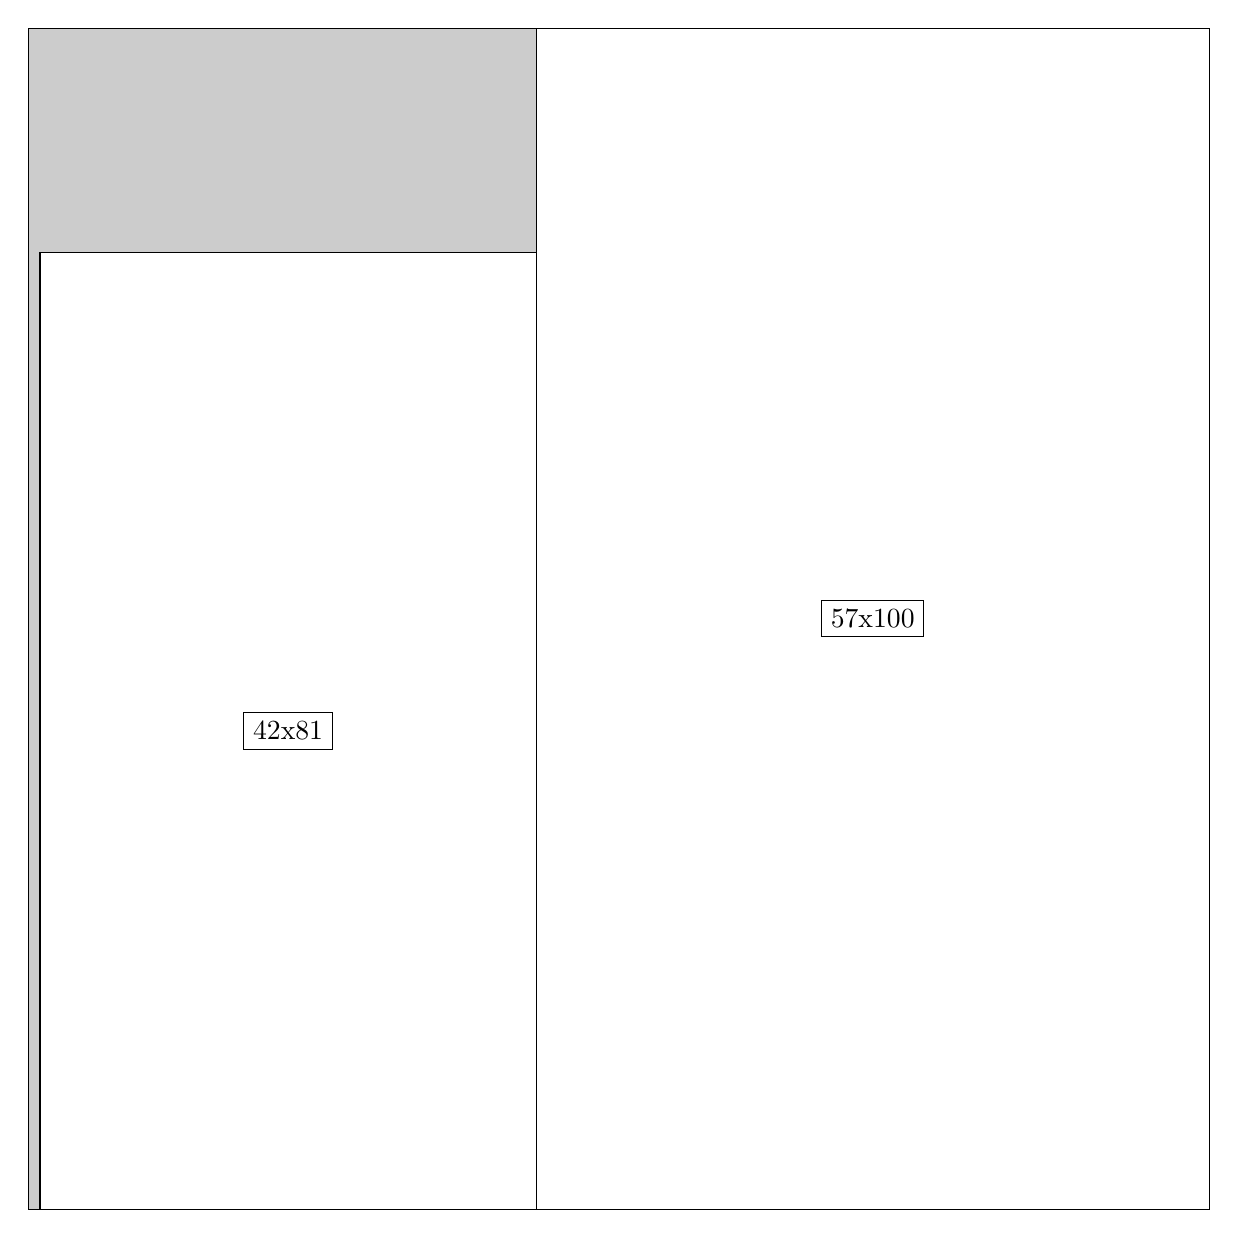
\begin{tikzpicture}[shorten >=1pt,scale=1.0,every node/.style={scale=1.0},->]
\tikzstyle{vertex}=[circle,fill=black!25,minimum size=14pt,inner sep=0pt]
\filldraw[fill=gray!40!white, draw=black] (0,0) rectangle (15.0,15.0);
\foreach \name/\x/\y/\w/\h in {57x100/6.45/0.0/8.549999999999999/15.0,42x81/0.15/0.0/6.3/12.15}
\filldraw[fill=white!40!white, draw=black] (\x,\y) rectangle node[draw] (\name) {\name} ++(\w,\h);
\end{tikzpicture}


w =57 , h =100 , x =43 , y =0 , v =5700
\par
w =42 , h =81 , x =1 , y =0 , v =3402
\par
\newpage


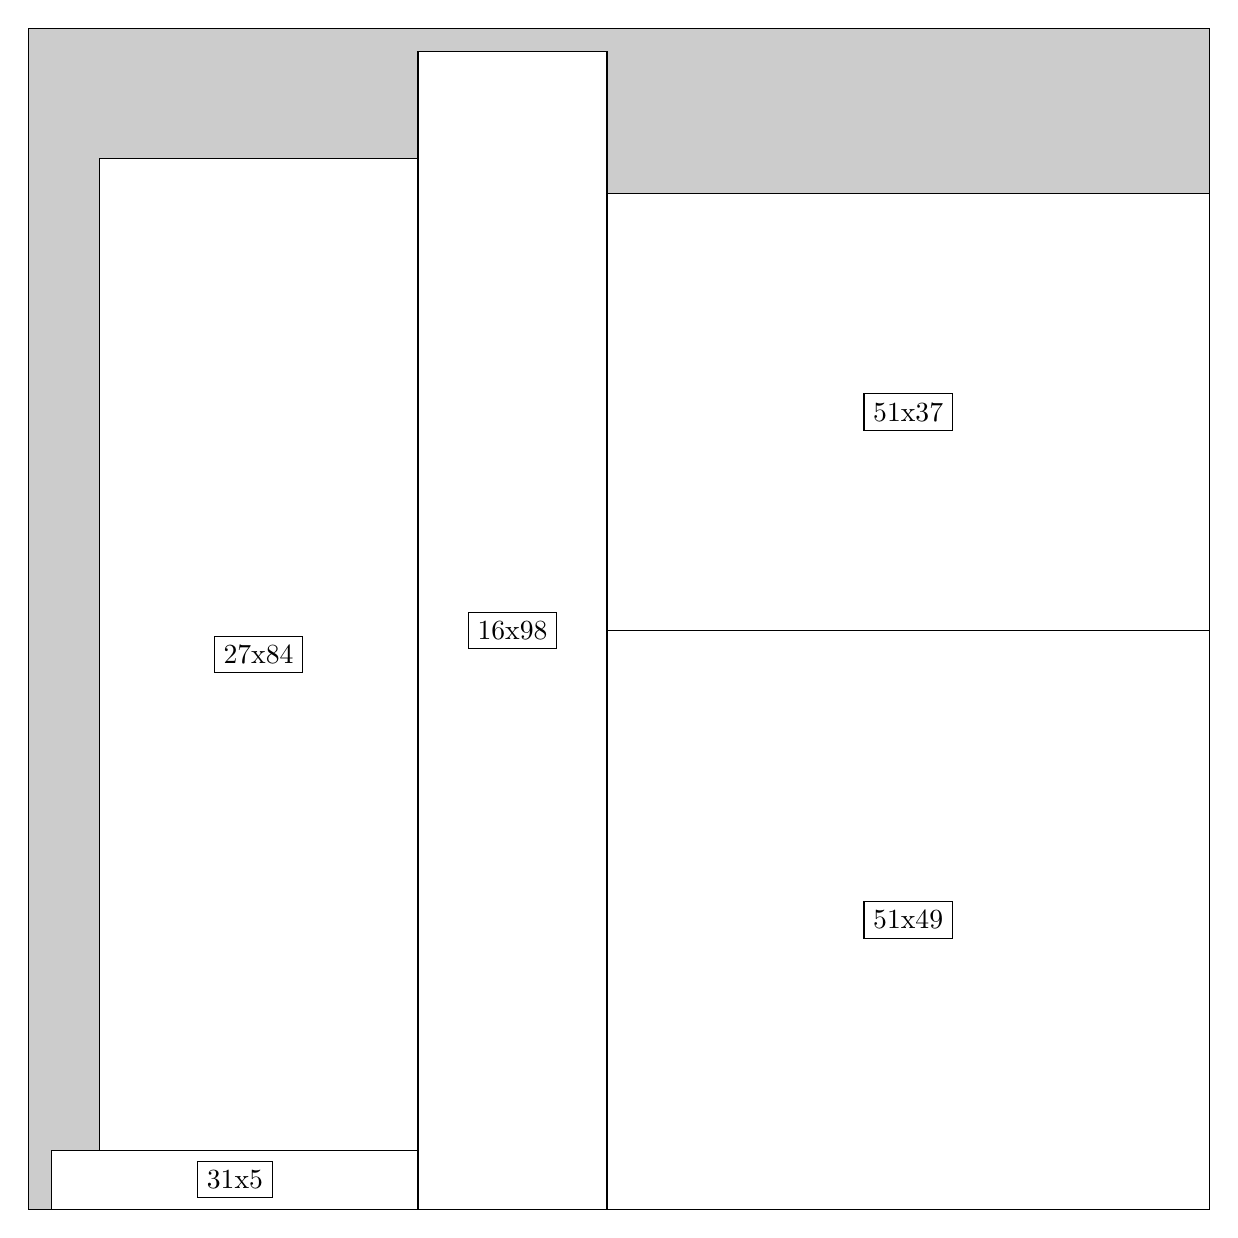
\begin{tikzpicture}[shorten >=1pt,scale=1.0,every node/.style={scale=1.0},->]
\tikzstyle{vertex}=[circle,fill=black!25,minimum size=14pt,inner sep=0pt]
\filldraw[fill=gray!40!white, draw=black] (0,0) rectangle (15.0,15.0);
\foreach \name/\x/\y/\w/\h in {51x49/7.35/0.0/7.6499999999999995/7.35,51x37/7.35/7.35/7.6499999999999995/5.55,16x98/4.95/0.0/2.4/14.7,31x5/0.3/0.0/4.6499999999999995/0.75,27x84/0.8999999999999999/0.75/4.05/12.6}
\filldraw[fill=white!40!white, draw=black] (\x,\y) rectangle node[draw] (\name) {\name} ++(\w,\h);
\end{tikzpicture}


w =51 , h =49 , x =49 , y =0 , v =2499
\par
w =51 , h =37 , x =49 , y =49 , v =1887
\par
w =16 , h =98 , x =33 , y =0 , v =1568
\par
w =31 , h =5 , x =2 , y =0 , v =155
\par
w =27 , h =84 , x =6 , y =5 , v =2268
\par
\newpage


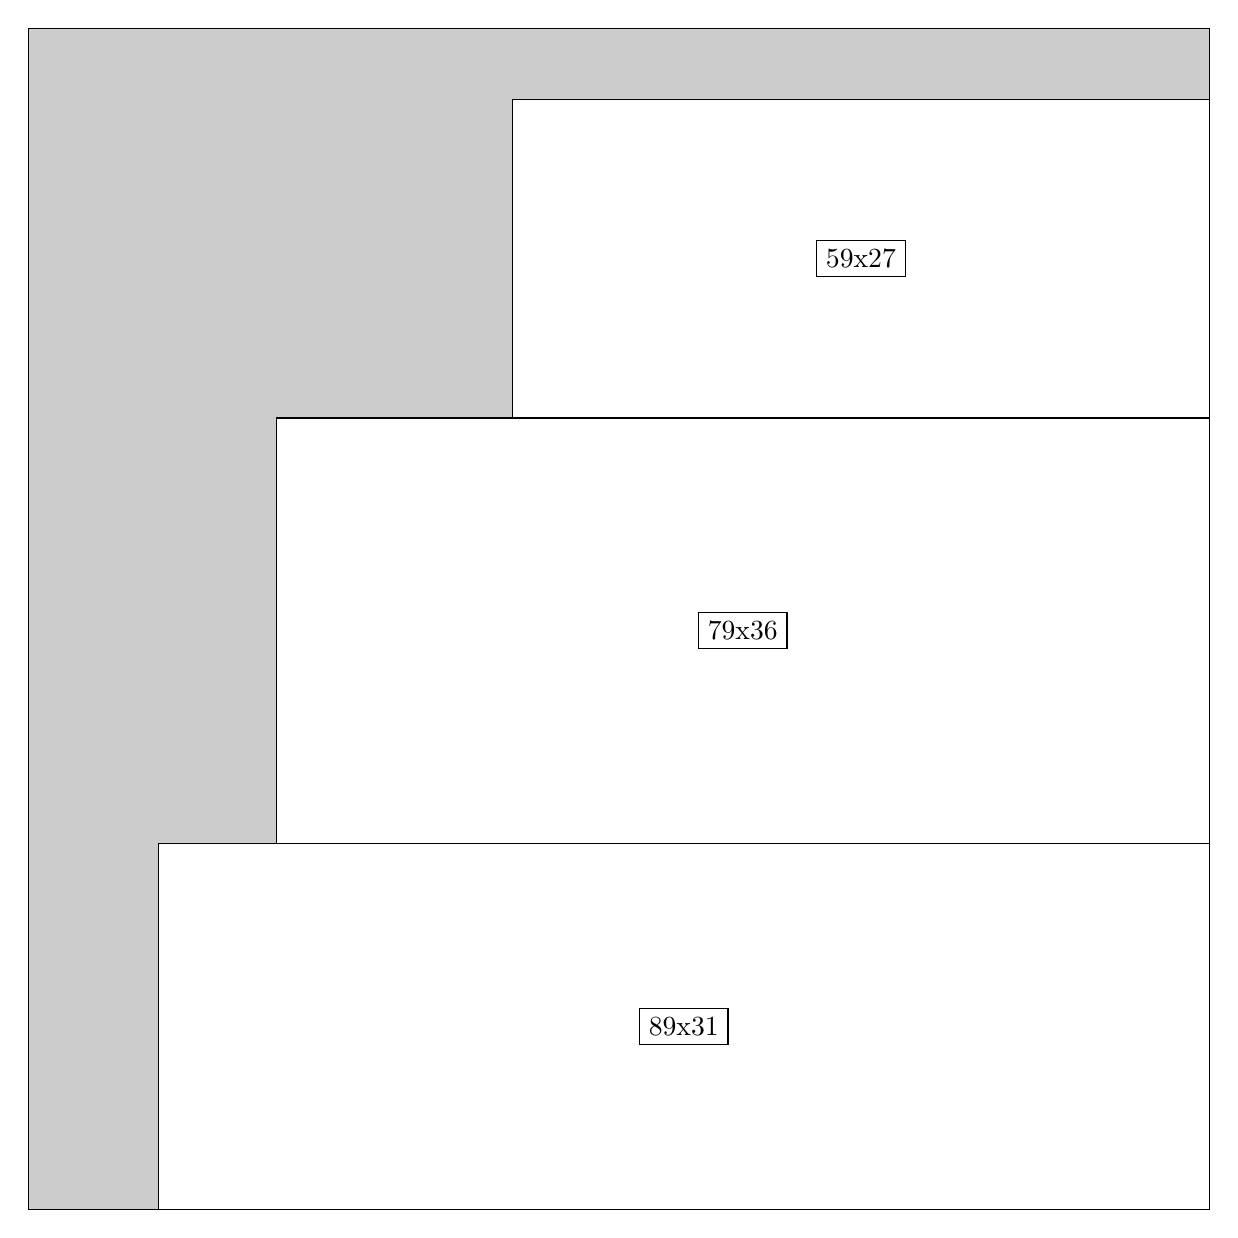
\begin{tikzpicture}[shorten >=1pt,scale=1.0,every node/.style={scale=1.0},->]
\tikzstyle{vertex}=[circle,fill=black!25,minimum size=14pt,inner sep=0pt]
\filldraw[fill=gray!40!white, draw=black] (0,0) rectangle (15.0,15.0);
\foreach \name/\x/\y/\w/\h in {89x31/1.65/0.0/13.35/4.6499999999999995,79x36/3.15/4.6499999999999995/11.85/5.3999999999999995,59x27/6.1499999999999995/10.049999999999999/8.85/4.05}
\filldraw[fill=white!40!white, draw=black] (\x,\y) rectangle node[draw] (\name) {\name} ++(\w,\h);
\end{tikzpicture}


w =89 , h =31 , x =11 , y =0 , v =2759
\par
w =79 , h =36 , x =21 , y =31 , v =2844
\par
w =59 , h =27 , x =41 , y =67 , v =1593
\par
\newpage


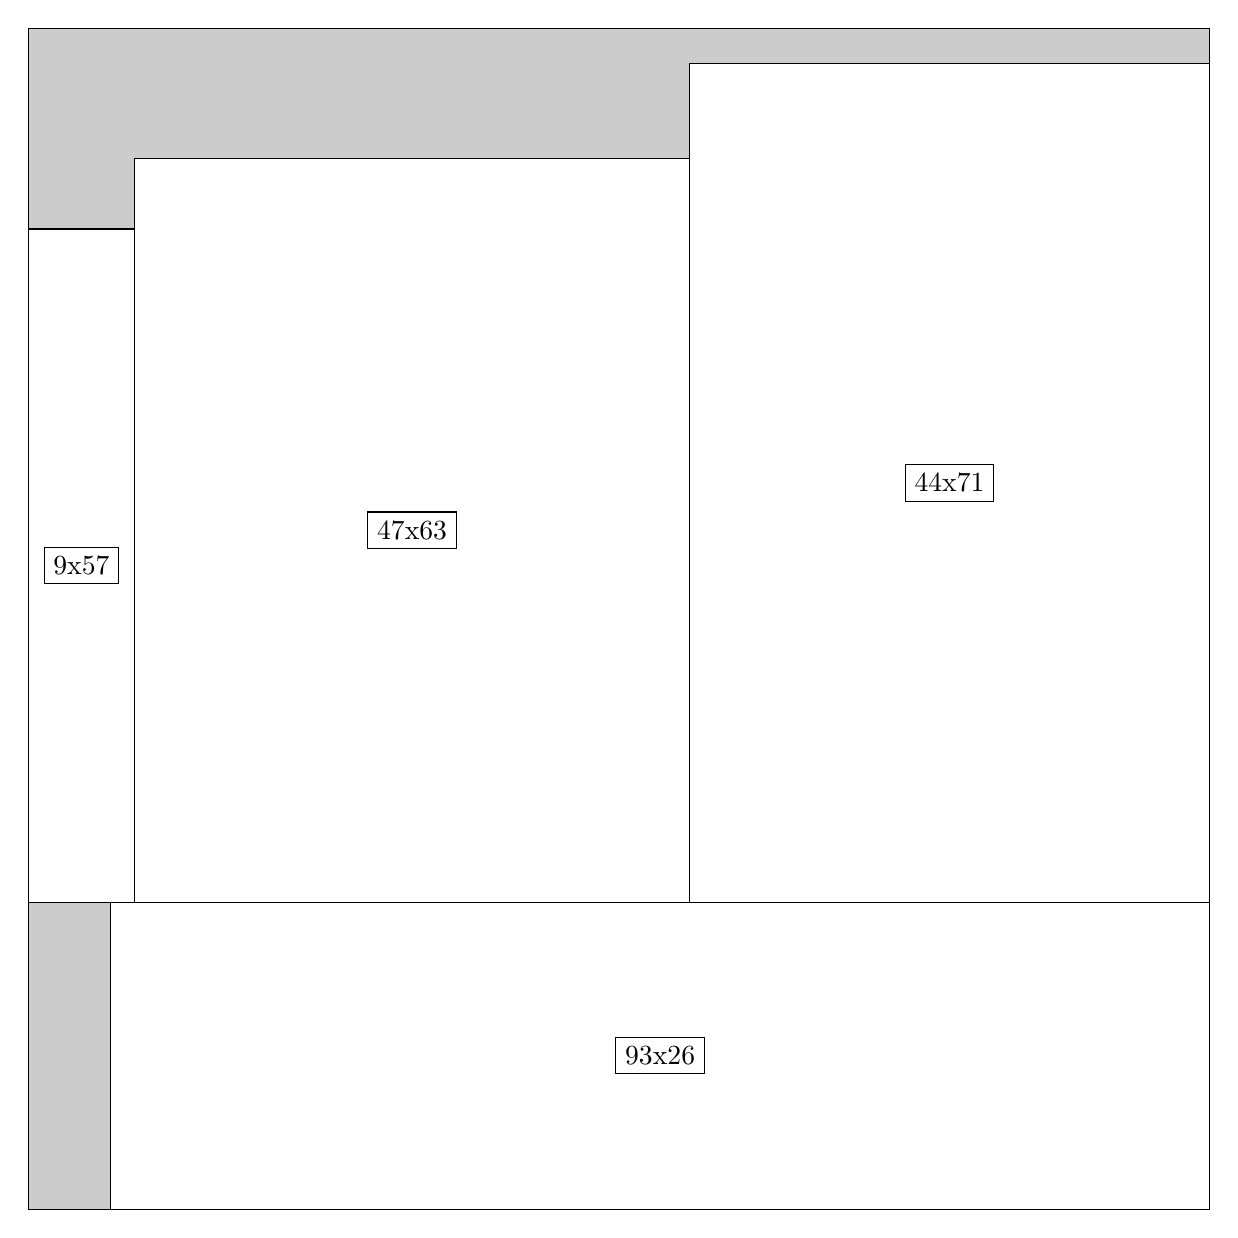
\begin{tikzpicture}[shorten >=1pt,scale=1.0,every node/.style={scale=1.0},->]
\tikzstyle{vertex}=[circle,fill=black!25,minimum size=14pt,inner sep=0pt]
\filldraw[fill=gray!40!white, draw=black] (0,0) rectangle (15.0,15.0);
\foreach \name/\x/\y/\w/\h in {93x26/1.05/0.0/13.95/3.9,44x71/8.4/3.9/6.6/10.65,47x63/1.3499999999999999/3.9/7.05/9.45,9x57/0.0/3.9/1.3499999999999999/8.549999999999999}
\filldraw[fill=white!40!white, draw=black] (\x,\y) rectangle node[draw] (\name) {\name} ++(\w,\h);
\end{tikzpicture}


w =93 , h =26 , x =7 , y =0 , v =2418
\par
w =44 , h =71 , x =56 , y =26 , v =3124
\par
w =47 , h =63 , x =9 , y =26 , v =2961
\par
w =9 , h =57 , x =0 , y =26 , v =513
\par
\newpage


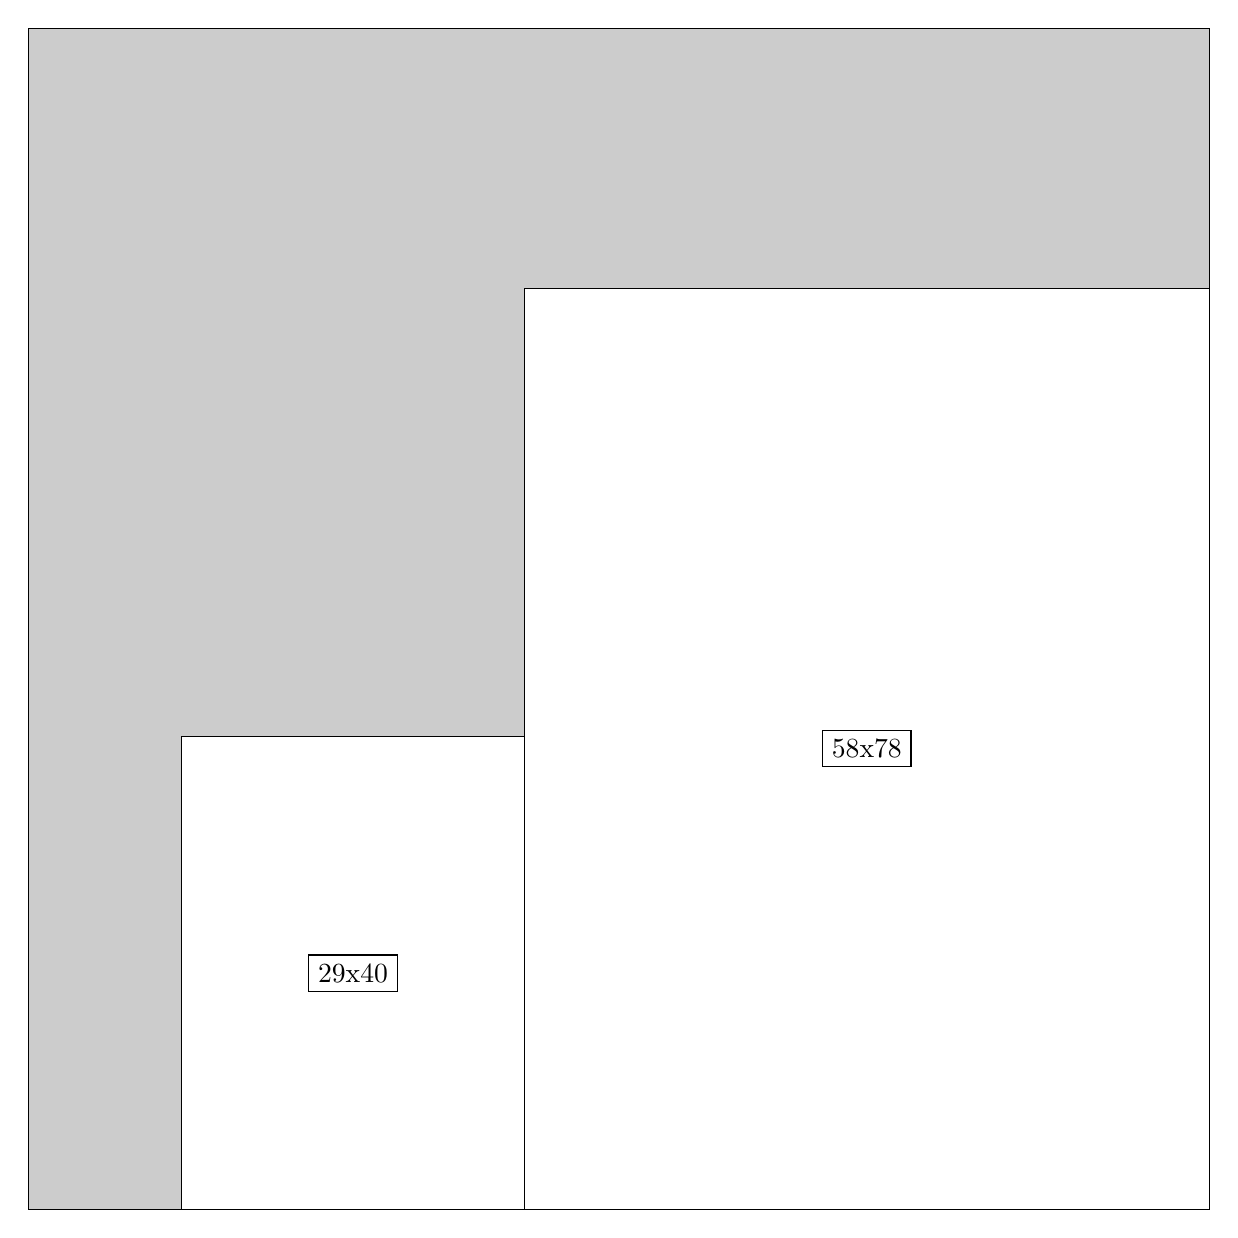
\begin{tikzpicture}[shorten >=1pt,scale=1.0,every node/.style={scale=1.0},->]
\tikzstyle{vertex}=[circle,fill=black!25,minimum size=14pt,inner sep=0pt]
\filldraw[fill=gray!40!white, draw=black] (0,0) rectangle (15.0,15.0);
\foreach \name/\x/\y/\w/\h in {58x78/6.3/0.0/8.7/11.7,29x40/1.95/0.0/4.35/6.0}
\filldraw[fill=white!40!white, draw=black] (\x,\y) rectangle node[draw] (\name) {\name} ++(\w,\h);
\end{tikzpicture}


w =58 , h =78 , x =42 , y =0 , v =4524
\par
w =29 , h =40 , x =13 , y =0 , v =1160
\par
\newpage


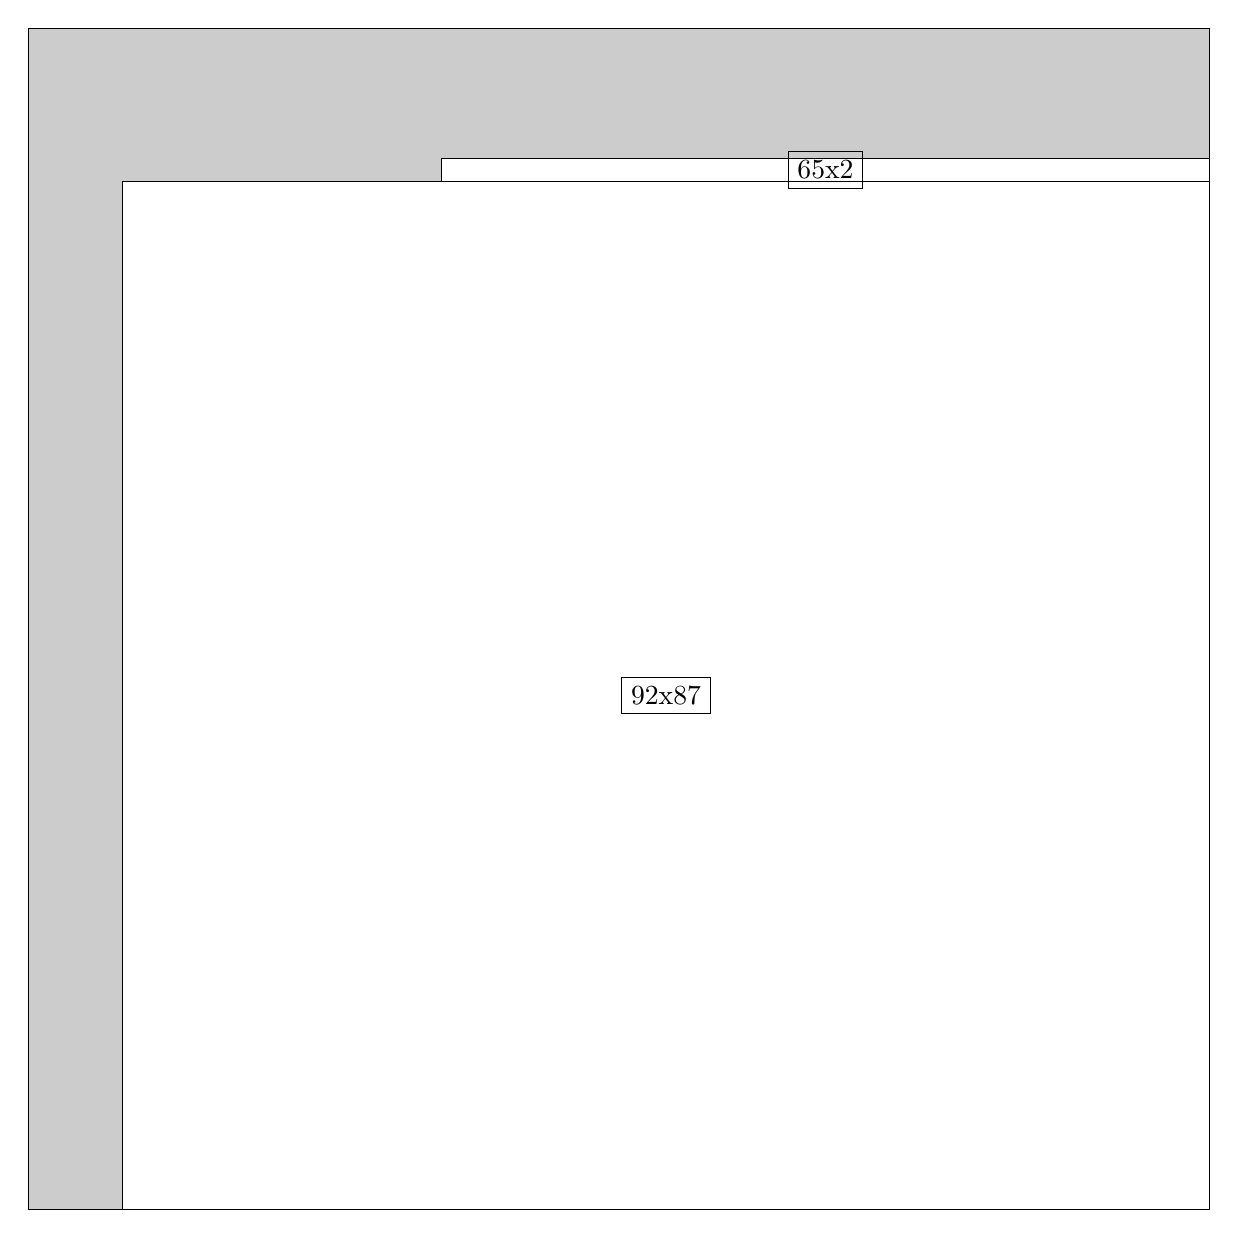
\begin{tikzpicture}[shorten >=1pt,scale=1.0,every node/.style={scale=1.0},->]
\tikzstyle{vertex}=[circle,fill=black!25,minimum size=14pt,inner sep=0pt]
\filldraw[fill=gray!40!white, draw=black] (0,0) rectangle (15.0,15.0);
\foreach \name/\x/\y/\w/\h in {92x87/1.2/0.0/13.799999999999999/13.049999999999999,65x2/5.25/13.049999999999999/9.75/0.3}
\filldraw[fill=white!40!white, draw=black] (\x,\y) rectangle node[draw] (\name) {\name} ++(\w,\h);
\end{tikzpicture}


w =92 , h =87 , x =8 , y =0 , v =8004
\par
w =65 , h =2 , x =35 , y =87 , v =130
\par
\newpage


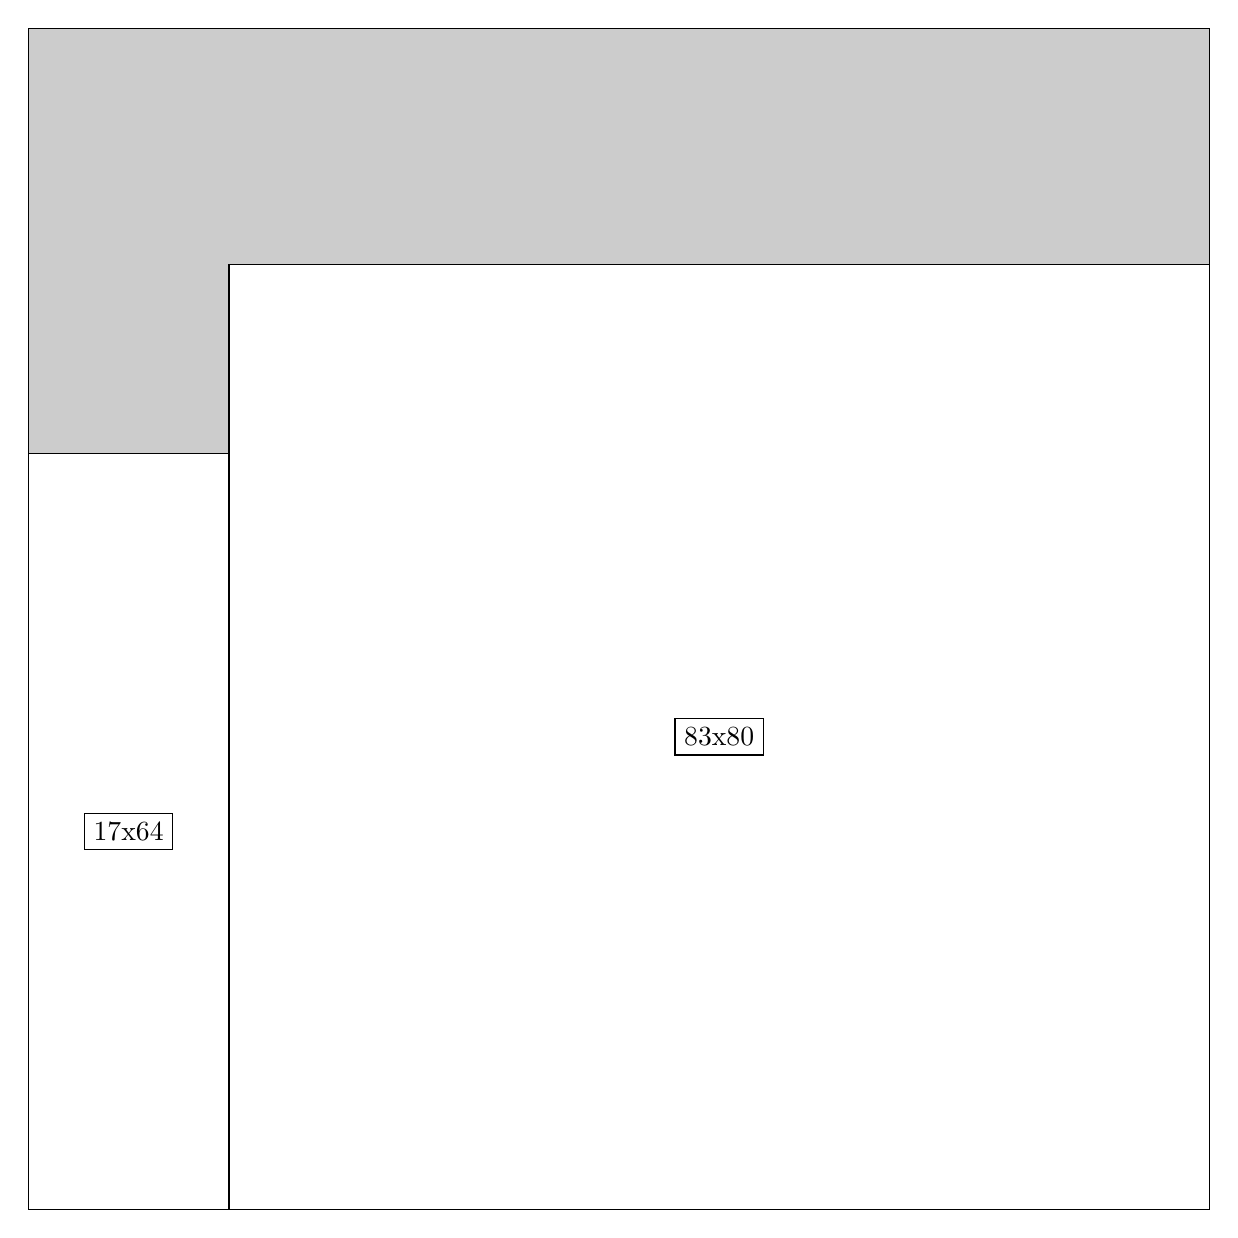
\begin{tikzpicture}[shorten >=1pt,scale=1.0,every node/.style={scale=1.0},->]
\tikzstyle{vertex}=[circle,fill=black!25,minimum size=14pt,inner sep=0pt]
\filldraw[fill=gray!40!white, draw=black] (0,0) rectangle (15.0,15.0);
\foreach \name/\x/\y/\w/\h in {83x80/2.55/0.0/12.45/12.0,17x64/0.0/0.0/2.55/9.6}
\filldraw[fill=white!40!white, draw=black] (\x,\y) rectangle node[draw] (\name) {\name} ++(\w,\h);
\end{tikzpicture}


w =83 , h =80 , x =17 , y =0 , v =6640
\par
w =17 , h =64 , x =0 , y =0 , v =1088
\par
\newpage


\end{document}